\documentclass[catalan]{scrartcl}

% encoding
\usepackage[utf8]{inputenc}
\usepackage[T1]{fontenc}
\usepackage{lmodern}
\usepackage{babel}

% formatting and fixes
\frenchspacing
\usepackage[style=spanish]{csquotes}
\MakeAutoQuote{«}{»}

% general design preferences (page, paragraph indent/space, margins, class options, ...)
\setlength{\parskip}{10pt}
\setlength{\parindent}{0pt}
%\pagestyle{plain}

% ADD ANY SPECIFIC PACKAGES HERE
% (CHEMISTRY, CODE, PUBLISHING)
\usepackage{siunitx}
\usepackage{tikz}
\usepackage{commath}
\usepackage{mathtools}
\usepackage{nicefrac}
\usepackage{minted}

% other options

%\usemintedstyle{xcode}
\setminted{
  %frame=leftline,
  %framesep=12pt,
  xleftmargin=15pt,
  breaklines,
  breakautoindent,
  breakindent=1em,
}

% hyperlink setup / metadata
\usepackage{hyperref}
\AfterPreamble{\hypersetup{
  pdftitle={Memòria P2 — PSAVC QP2019},
  %pdfsubject={PSAVC},
}}

% document metadata
\author{Alba Mendez}
\title{Memòria pràctica 2\\
{\small PSAVC QP2019}}
\date{23 d'abril de 2019}

\begin{document}

%\begin{minipage}{\columnwidth}
\maketitle
%\end{minipage}


\part{Estudi previ}

\paragraph{Qüestió 1.1.}

El nombre de gols que marca un equip ($g$) es pot modelar com una V.A. de
Poisson amb la distribució següent:
%
\begin{equation}
  P(g) = \frac{\lambda^g \, e^{-\lambda} }{g!}, \quad g = 0,1,2,\hdots
\end{equation}
%
Cal demostrar que $E\{g\} = \lambda$ i $E\{(g - \lambda)^2\} = \lambda$.

Per fer la primera demostració fem el sumatori sobre tots els valors,
i tenint en compte que $\sum^{\infty}_{n=0} \lambda \frac{\lambda^n}{n!}$
és la sèrie de Taylor de $\lambda e^\lambda$:
%
\begin{align}
  E\{g\} &= \sum^{\infty}_{g=-\infty} g \, P(g)
\\
  E\{g\} &= \sum^{\infty}_{g=0} g \frac{\lambda^g \, e^{-\lambda} }{g!}
\\
  E\{g\} &= e^{-\lambda} \, \sum^{\infty}_{g=1} g \frac{\lambda^g }{g!}
\\
  E\{g\} &= e^{-\lambda} \, \sum^{\infty}_{g=1} \frac{\lambda^g }{(g-1)!}
\\
  E\{g\} &= e^{-\lambda} \, \sum^{\infty}_{g=0} \frac{\lambda^{g+1} }{g!}
\\
  E\{g\} &= e^{-\lambda} \, \lambda e^\lambda
\\
  E\{g\} &= \lambda
\end{align}
%
Queda demostrat. Ara, per a la segona demostració fem servir
$E\{(X - E\{X\})^2\} = E\{X^2\} - E\{X\}^2$ i tenint en compte que
$\sum^{\infty}_{n=0} \lambda^2 \frac{\lambda^n}{n!}$ és la sèrie de Taylor
de $\lambda^2 e^\lambda$:
%
\begin{align}
  E\{(g - \lambda)^2\} &= E\{ g^2 \} - \lambda^2
\\
  E\{(g - \lambda)^2\} &= \left[ \sum^\infty_{g=-\infty} g^2
    P(g) \right] - \lambda^2
\\
  E\{(g - \lambda)^2\} &= e^{-\lambda} \, \left[ \sum^\infty_{g=0} g^2
    \frac{\lambda^g }{g!} \right] - \lambda^2
\\
  E\{(g - \lambda)^2\} &= e^{-\lambda} \, \left[ \sum^\infty_{g=1} g
    \frac{\lambda^g }{(g-1)!} \right] - \lambda^2
%
\\
  E\{(g - \lambda)^2\} &= e^{-\lambda} \, \left[ \sum^\infty_{g=1} [(g-1) + 1]
    \frac{\lambda^g }{(g-1)!} \right] - \lambda^2
\\
  E\{(g - \lambda)^2\} &= e^{-\lambda} \, \left[ \sum^\infty_{g=2}
    \frac{\lambda^g }{(g-2)!} +
    \sum^\infty_{g=1} \frac{\lambda^g }{(g-1)!} \right] - \lambda^2
\\
  E\{(g - \lambda)^2\} &= e^{-\lambda} \, \left[ \lambda^2 e^\lambda +
    \lambda e^\lambda \right] - \lambda^2
\\
  E\{(g - \lambda)^2\} &= \lambda
%
\end{align}

\paragraph{Qüestió 1.2.}

Cal trobar la mitjana, la variància i l'error quadràtic mig dels
tres estimadors esmentats.

Tots els estimadors son una combinació lineal de les variables
($\mathbf{v}^T \cdot \mathbf{g}$). La esperança és lineal, per tant
$E\{ \mathbf{v}^T \cdot \mathbf{g} \} \Leftrightarrow
\mathbf{v}^T \cdot E\{\mathbf{g}\} \Leftrightarrow
\mathbf{v}^T \cdot \lambda\mathbf{1}$.
A més les variables són incorrelades, per tant
$Var\{ \mathbf{v}^T \cdot \mathbf{g} \}
\Leftrightarrow \sum_{i=1}^N v_i^2 \cdot Var\{g_i\} \Leftrightarrow
\lambda \sum_{i=0}^N v_i^2$.

Per a l'estimador $\hat{\lambda}_A^N$, $\mathbf{v} =
\frac{2}{N(N+1)} \mathbf{n}$:
%
\begin{align}
  E\{\hat{\lambda}_A^N\} &= \lambda \frac{2}{N(N+1)} \sum_{n=1}^N n = \lambda
\\
  Var\{\hat{\lambda}_A^N\} &= \lambda \frac{4}{N^2(N+1)^2}
    \sum_{n=1}^N n^2
    = \lambda \frac{2(2N+1)}{3N(N+1)}
\end{align}
%
Per a l'estimador $\hat{\lambda}_B^N$, $\mathbf{v} =
\frac{1}{N} \mathbf{1}$:
%
\begin{align}
  E\{\hat{\lambda}_B^N\} &= \lambda \frac{1}{N} N = \lambda
\\
  Var\{\hat{\lambda}_B^N\} &= \lambda \frac{1}{N^2} N
    = \frac{\lambda}{N}
\end{align}
%
Per a l'estimador $\hat{\lambda}_C^N$, $\mathbf{v} =
\frac{1}{2N} \mathbf{1}$:
%
\begin{align}
  E\{\hat{\lambda}_C^N\} &= \lambda \frac{1}{2N} N = \frac{\lambda}{2}
\\
  Var\{\hat{\lambda}_C^N\} &= \lambda \frac{1}{4N^2} N
    = \frac{\lambda}{4N}
\end{align}
%
Els primers dos estimadors són no esbiaixats, per tant l'MSE és igual a la
variància. En l'últim, el biaix és $\frac{\lambda}{2}$ i l'MSE és
$\frac{\lambda}{4N} + \frac{\lambda^2}{4} = \frac{\lambda}{4} (\frac{1}{N} + \lambda)$.

\paragraph{Qüestió 1.3.}

Cal trobar la funció de \emph{log-likelihood} del problema i obtenir la cota de
Cramér-Rao, i determinar si algun dels estimadors anteriors és eficient.

La funció de \emph{log-likelihood} és:
%
\begin{align}
  \ell(\mathbf{g};\lambda) &= \ln P(\mathbf{g};\lambda) =
    \ln \prod_{i=1}^N \frac{\lambda^{g_i} e^{-\lambda}}{g_i!}
\\
  \ell(\mathbf{g};\lambda) &=
    \sum_{i=1}^N \ln \frac{\lambda^{g_i} e^{-\lambda}}{g_i!}
\\
  \ell(\mathbf{g};\lambda) &=
    \sum_{i=1}^N g_i \ln \lambda -\lambda - \ln g_i!
\\
  \ell(\mathbf{g};\lambda) &=
    -\lambda + \ln \lambda \sum_{i=1}^N g_i - \sum_{i=1}^N \ln g_i!
\end{align}
%
La cota de Cramér-Rao és:
%
\begin{align}
  CRB &= \left[ -E\left\{ \pd[2]{}{\lambda} \ell(\mathbf{g};\lambda) \right\} \right]^{-1}
\\
  CRB &= \left[ -E\left\{ \pd[2]{}{\lambda}
    \left(-\lambda + \ln \lambda \sum_{i=1}^N g_i - \sum_{i=1}^N \ln g_i! \right)
  \right\} \right]^{-1}
\\
  CRB &= \left[ -E\left\{ \left(\sum_{i=1}^N g_i\right) \pd[2]{}{\lambda}
    \ln \lambda
  \right\} \right]^{-1}
\\
  CRB &= \left[ E\left\{ \sum_{i=1}^N g_i
  \right\} \cdot \frac{1}{\lambda^2} \right]^{-1}
\\
  CRB &= \left[ \frac{N}{\lambda} \right]^{-1} = \frac{\lambda}{N}
\end{align}
%
Per tant, l'estimador $\hat{\lambda}_B^N$ és eficient.


\part{Activitat al laboratori}

\paragraph{Activitat 1.1.}

Fixant el paràmetre a estimar $\lambda = 2$, cal simular el nombre de gols
que ha marcat l'equip en els últims $N = 20$ partits. Per fer-ho, generem
un vector de $N$ mostres de Poisson mitjançant \mintinline{matlab}|poissrnd|:

\begin{minted}{matlab}
lambda = 2;
N = 20;
g = poissrnd(ones(N,1) * lambda);
\end{minted}

\paragraph{Activitat 1.2.}

Ara es demana visualitzar l'histograma d'aquestes mostres i comparar-ho amb
la distribució teòrica, que imprimirem amb una línia:

\begin{minted}{matlab}
gs = 0:max(g);
hist(g, gs);
plot(gs, N * lambda.^gs * exp(-lambda) ./ factorial(gs));
\end{minted}

\begin{figure}
\center
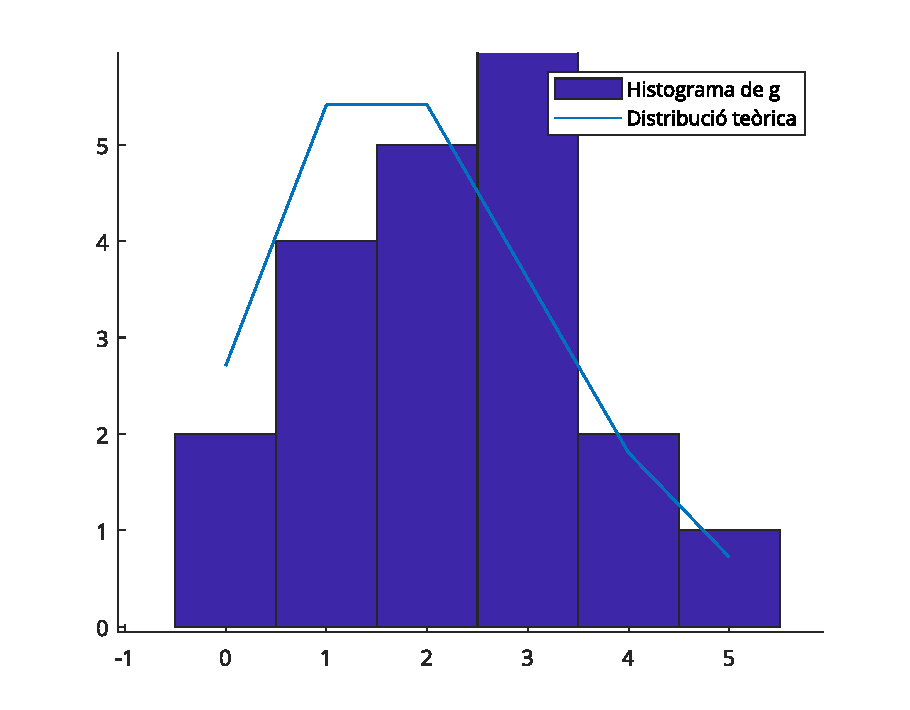
\includegraphics[width=\textwidth]{../fig1.pdf}
\caption{Histograma dels gols marcats $g_i$, comparat amb la probabilitat teòrica. \label{fig:fig1}}
\end{figure}

Es pot veure una realització (independent a la resta d'activitats) del resultat a la figura~\ref{fig:fig1}.

No se gaire de futbol, però dubto que els resultats del partit siguin realment
independents, com a mínim s'hauria de comptar com a factor si l'equip juga a
casa seva o del rival.

\paragraph{Activitat 1.3.}

Ara es demana aplicar els tres estimadors a les mostres simulades:

\begin{minted}{matlab}
lambda_a = 2/(N*(N+1)) * (1:N) * g
lambda_b = sum(g) / N
lambda_c = sum(g) / (2*N)
\end{minted}

Les estimacions (per a una realització independent a la resta d'activitats) són:\\
$\hat{\lambda}_A = 2.3952; \hat{\lambda}_B = 2.2000; \hat{\lambda}_C = 1.1000$.
S'aprecia com l'estimador proposat per l'estudiant B (estimador eficient) s'apropa més al
valor real del paràmetre, i això es repeteix en la majoria de realitzacions.

\paragraph{Activitat 1.4.}

A continuació es demana representar, en funció de $N$, el CRB juntament amb
els MSE i variàncies teòriques de cada estimador. Cal representar de $N = 1$ fins
a $20$.

Com que el CRB coincideix amb l'MSE
de $\hat{\lambda}_B^N$, ens limitarem a representar els tres MSEs (ressaltant
el de l'estimador eficient) segons les expressions de l'estudi previ:

\begin{minted}{matlab}
N = 1:20;
plot(lambda * (2*(2*N + 1)) ./ (3*N.*(N + 1)), 'Color', colors{1});
plot(lambda ./ N, 'LineWidth', 2, 'Color', colors{2});
plot(lambda ./ (4*N) + lambda^2 / 4, 'Color', colors{3});
\end{minted}

On \mintinline{matlab}|colors| és un array definit amb antelació. Ara només
queda imprimir les variàncies, i en concret només cal imprimir la de $\hat{\lambda}_C^N$
ja que en la resta coincideix amb l'MSE:

\begin{minted}{matlab}
plot(lambda ./ (4*N), 'Color', [.5 .5 .5]);
\end{minted}

\begin{figure}
\center
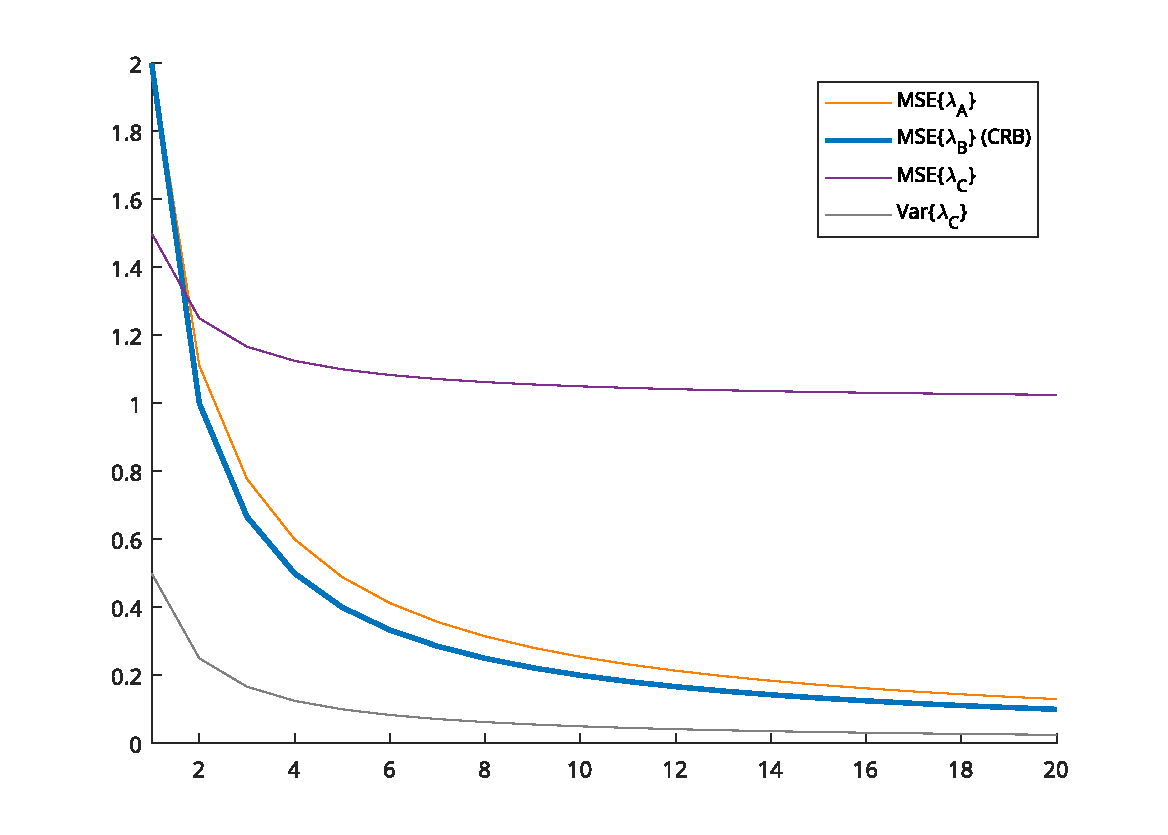
\includegraphics[width=\textwidth]{../fig2-1.pdf}
\caption{MSE i variància teòrica de cada estimador en funció de $N$. \label{fig:fig2-1}}
\end{figure}

El resultat es pot veure a la figura~\ref{fig:fig2-1}. Es confirma, doncs,
que l'estimador eficient ($\hat{\lambda}_B$) és en general la millor tria.

\paragraph{Activitat 1.5.}

Ara s'han de simular, per a cada valor de $N$, $R = 1000$ realitzacions de $\mathbf{g}$
i aplicar els tres estimadors a cada realització. A partir d'això cal representar la corba de MSE de les
estimacions.

Començarem simulant les realitzacions. Les desarem en una matriu on la
primera dimensió és $N$, la segona és $R$ i la tercera és l'estimador (1 = A, 2 = B, 3 = C):

\begin{minted}{matlab}
R = 1000;
lambdas = [];
for N = 1:20
    g = poissrnd(ones(N,R) * lambda);
    lambdas(N,:,1) = 2/(N*(N+1)) * (1:N) * g;
    lambdas(N,:,2) = sum(g, 1) / N;
    lambdas(N,:,3) = sum(g, 1) / (2*N);
end
\end{minted}

Un cop tenim les estimacions simulades, per a cada estimador calculem la seva
corba d'MSE empíric i la representem sobre el gràfic anterior (amb el mateix
color que la corba teòrica, però fent servir creus en comptes d'una línia sòlida):

\begin{minted}{matlab}
for i = 1:3
    plot(mse(lambdas(:,:,i)', lambda), 'x', 'Color', colors{i});
end
\end{minted}

\begin{figure}
\center
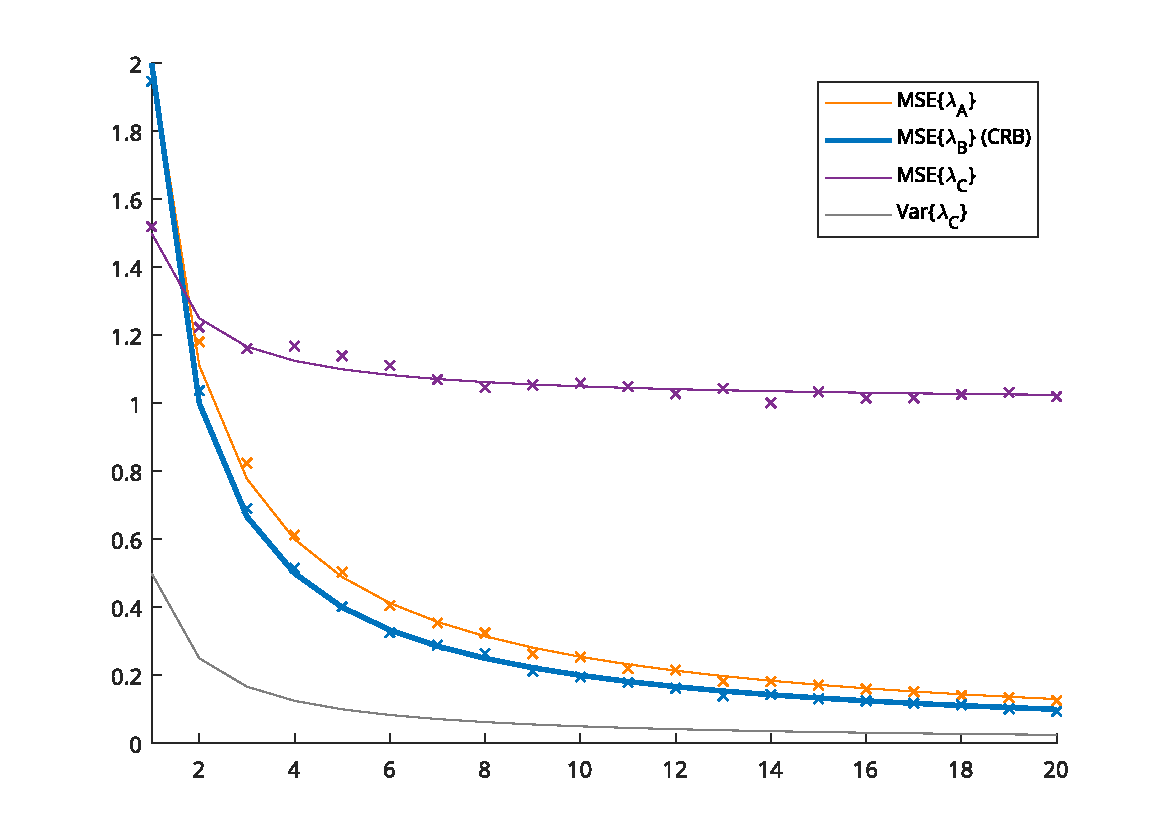
\includegraphics[width=\textwidth]{../fig2-2.pdf}
\caption{Comparativa dels MSE teòrics (línia) i empírics (creus) de cada estimador, en funció de $N$. \label{fig:fig2-2}}
\end{figure}

On \mintinline{matlab}|mse(x_e, x)| es defineix com \mintinline{matlab}|mean((x_e - x).^2)|.
El gràfic resultant (per a una realització independent a la resta d'activitats) es pot veure
a la figura~\ref{fig:fig2-2}. Es comprova com l'MSE empíric s'ajusta al teòric. Per a valors
molt petits de $N$, l'ajust no és tan bo.

\paragraph{Activitat 1.6.}

Per últim, cal considerar que en realitat el valor estimat s'acabaria arrodonint
a l'enter més proper. Cal representar el MSE empíric però ara tenint en compte l'error
d'aquest arrodoniment.

Per fer-ho, només ens cal repetir l'últim pas de l'activitat anterior, però aplicant
\mintinline{matlab}|round| a la matriu d'estimacions abans de calcular-ne la corba MSE.

Per tant, afegim aquesta línia al bucle anterior (ara usem
aspes en comptes de creus):

\begin{minted}{matlab}
plot(mse(round(lambdas(:,:,i))', lambda), '*', 'Color', colors{i});
\end{minted}

\begin{figure}
\center
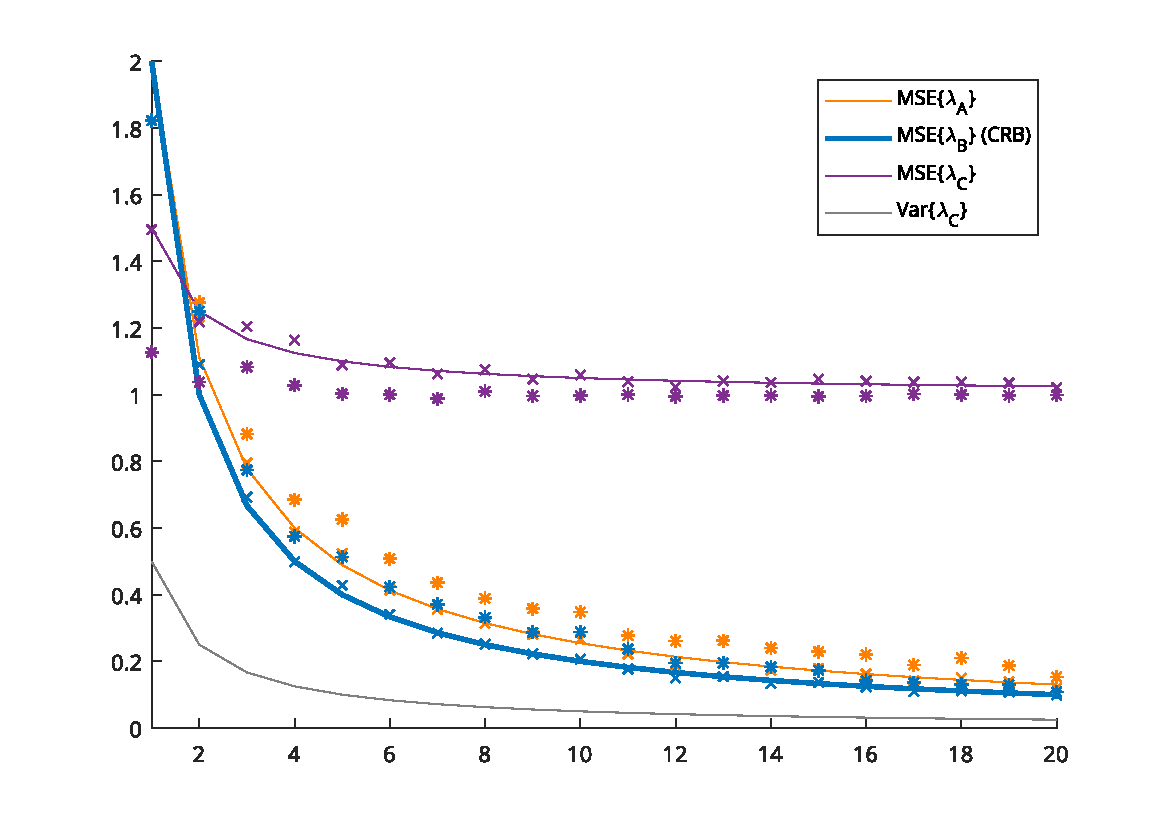
\includegraphics[width=\textwidth]{../fig2-3.pdf}
\caption{Comparativa dels MSE teòrics (línia), empírics (creus) i empírics
considerant l'arrodoniment (aspes) de cada estimador, en funció de $N$. \label{fig:fig2-3}}
\end{figure}

El gràfic resultant (per a una realització independent a la resta d'activitats) es pot veure
a la figura~\ref{fig:fig2-3}.
Cal destacar que l'arrodoniment \emph{millora} l'MSE en l'estimador esbiaixat (pel pes de
l'arrodoniment cap a dalt),
mentre que als altres estimadors l'empitjora. També s'observa com, a mida que $N$ creix,
l'impacte de l'arrodoniment es redueix i els dos MSE s'apropen. Per a $N = 20$ és molt petit,
tot i que no del tot negligible. Per últim, tenir en compte que l'impacte de l'arrodoniment
en l'MSE també es reduiria si $\lambda$ augmentés.

\clearpage
\part*{Annex. Codi MATLAB}

%El codi emprat per a la realització de la pràctica es troba a continuació:

\begin{minted}{matlab}
%% Activitat 1

lambda = 2;
N = 20;
g = poissrnd(ones(N,1) * lambda);

%% Activitat 2

gs = 0:max(g);
figure(1); cla; hold on
hist(g, gs);
plot(gs, N * lambda.^gs * exp(-lambda) ./ factorial(gs));
legend('Histograma de g', 'Distribució teòrica');

%% Activitat 3

lambda_a = 2/(N*(N+1)) * (1:N) * g
lambda_b = sum(g) / N
lambda_c = sum(g) / (2*N)

%% Activitats 4, 5, 6

N = 1:20;
figure(2); cla; hold on
colors = { [1 .5 0], [0 .45 .74], [.5 0.18 0.56] };
xlim([N(1) N(end)]);

plot(lambda * (2*(2*N + 1)) ./ (3*N.*(N + 1)), 'Color', colors{1});
plot(lambda ./ N, 'LineWidth', 2, 'Color', colors{2});
plot(lambda ./ (4*N) + lambda^2 / 4, 'Color', colors{3});
plot(lambda ./ (4*N), 'Color', [.5 .5 .5]);

R = 1000;
lambdas = [];
for N = 1:20
    g = poissrnd(ones(N,R) * lambda);
    lambdas(N,:,1) = 2/(N*(N+1)) * (1:N) * g;
    lambdas(N,:,2) = sum(g, 1) / N;
    lambdas(N,:,3) = sum(g, 1) / (2*N);
end

for i = 1:3
    plot(mse(lambdas(:,:,i)', lambda), 'x', 'Color', colors{i});
    plot(mse(round(lambdas(:,:,i))', lambda), '*', 'Color', colors{i});
end

legend('MSE\{\lambda_A\}', 'MSE\{\lambda_B\} (CRB)', 'MSE\{\lambda_C\}', 'Var\{\lambda_C\}');

%% Utilitats

function e = mse(x_e, x)
    e = mean((x_e - x).^2);
end
\end{minted}


\end{document}
